% Copyright (c) 2021 Tobias Briones. All rights reserved.
% SPDX-License-Identifier: CC-BY-4.0
%
% This file is part of https://github.com/tobiasbriones/
% cp-unah-mm700-agricultural-soil-sampling-for-data-analysis
%
% This source code is licensed under the Creative Commons Attribution 4.0
% International License found in the LICENSE-CC file in the root directory of
% this source tree or at https://spdx.org/licenses/CC-BY-4.0

\subsection{Patrones de Muestreo}

Un patrón de muestreo se puede aplicar por ejemplo, a cada estrato de un muestreo estratificado. En el caso más trivial se puede hacer referencia a un patrón aleatorio, en otros casos se puede utilizar uno más elaborado. Esta sección recopila los patrones de muestreos de acuerdo a la \textit{Guía de muestreo de suelo $\mid$ Gob.Pe} \cite{gobpe-ministerio-del-ambiente-2014}.

\bigbreak

Los patrones de muestreo se clasifican de acuerdo a si son:  con distribución aleatoria, con distribución uniforme, con distribución heterogénea.

\subsubsection{Con Distribución Aleatoria}

Estos patrones de muestreo son utilizados en estadística.

\bigbreak

\textbf{Aleatorio:} Los puntos se escogen de forma aleatoria. Los resultados son muy irregulares.

\bigbreak

\textbf{Aleatorio sobre rejilla regular (estratificado):} El plano se divide (particiona) en zonas (estratos), se delimita una rejilla regular en todo el plano y se escoge un número igual de puntos distribuidos aleatoriamente en cada celda. Ya se ha hablado a más detalle de este patrón en secciones anteriores. La desventaja es que la forma en que están distribuidos los puntos puede ser muy dispersa, estando unos muy cerca y otros muy lejos por lo que quedan brechas de espacio vacío a menudo.

\bigbreak

\textbf{Aleatorio desalineado sobre rejilla regular:} Es una variante del patrón estratificado. En algunas celdas, la coordenada \say{x} se mueve al azar y en el resto de las celdas se mueve la coordenada \say{y}, o viceversa. La desventaja también se hereda del método estratificado.

\begin{figure}[H]
    \centering
    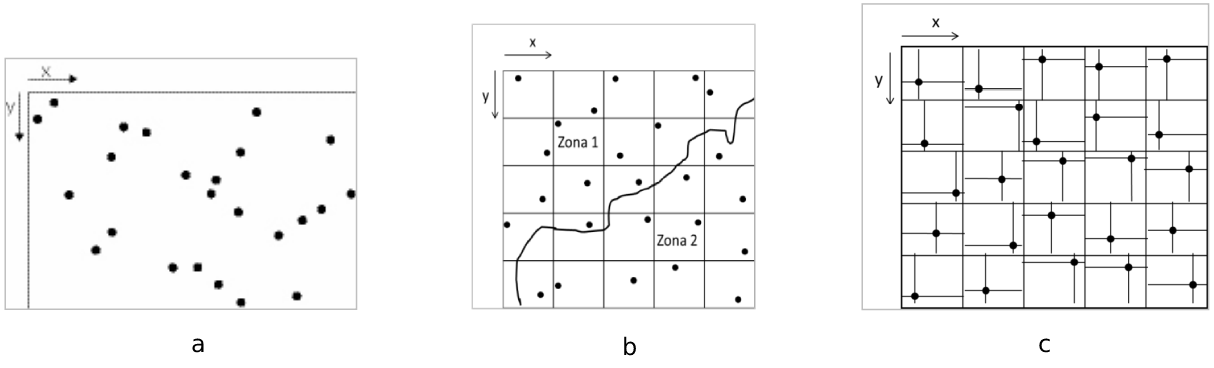
\includegraphics[width=0.3\paperwidth]{ref/random-sampling-patterns.png}
    \caption{Patrones de muestreo con distribución aleatoria}
    a) Aleatorio, b) Aleatorio sobre rejilla regular, c) Aleatorio desalineado sobre rejilla regular \\
    Fuente: \textit{Guía de muestreo de suelo $\mid$ Gob.Pe} \cite{gobpe-ministerio-del-ambiente-2014}
\end{figure}

\subsubsection{Con Distribución Uniforme}

\textbf{Rejillas regulares:} Se hace una rejilla de cuadrados en el plano donde cada celda es tan grande como se necesite (inversamente proporcionalmente al nivel de detalle). Por último se escoge el punto en cualquier parte de \textit{cada} celda verificando que la posición del punto sea la misma en todas las celdas.

\bigbreak

\textbf{Rejillas triangulares:} Se trazan triángulos equiláteros en el plano y se aplica el nivel de detalle establecido arriba.

\bigbreak

\textbf{Rejilla circular:} Para análisis de contaminación es de utilidad para delimitar la zona contaminada. Se trazan círculos concéntricos, separados de acuerdo al detalle requerido. Se trazan líneas rectas considerando los 8 puntos cardinales principales y se ubican los puntos de muestreo en las intersecciones. Se espera que con esta rejilla las mayores concentraciones de contaminantes se ubiquen en el centro.

\bigbreak

\textbf{Sobre una línea:} Este patrón también sirve para contaminantes cuando la contaminación siga una línea recta.

\bigbreak

\textbf{Diagonales múltiples:} Por último, con este patrón se traza una diagonal central y líneas paralelas en el plano, sobre las cuales se ubican los puntos de muestreo, manteniendo la misma distancia entre ellos.

\begin{figure}[H]
    \centering
    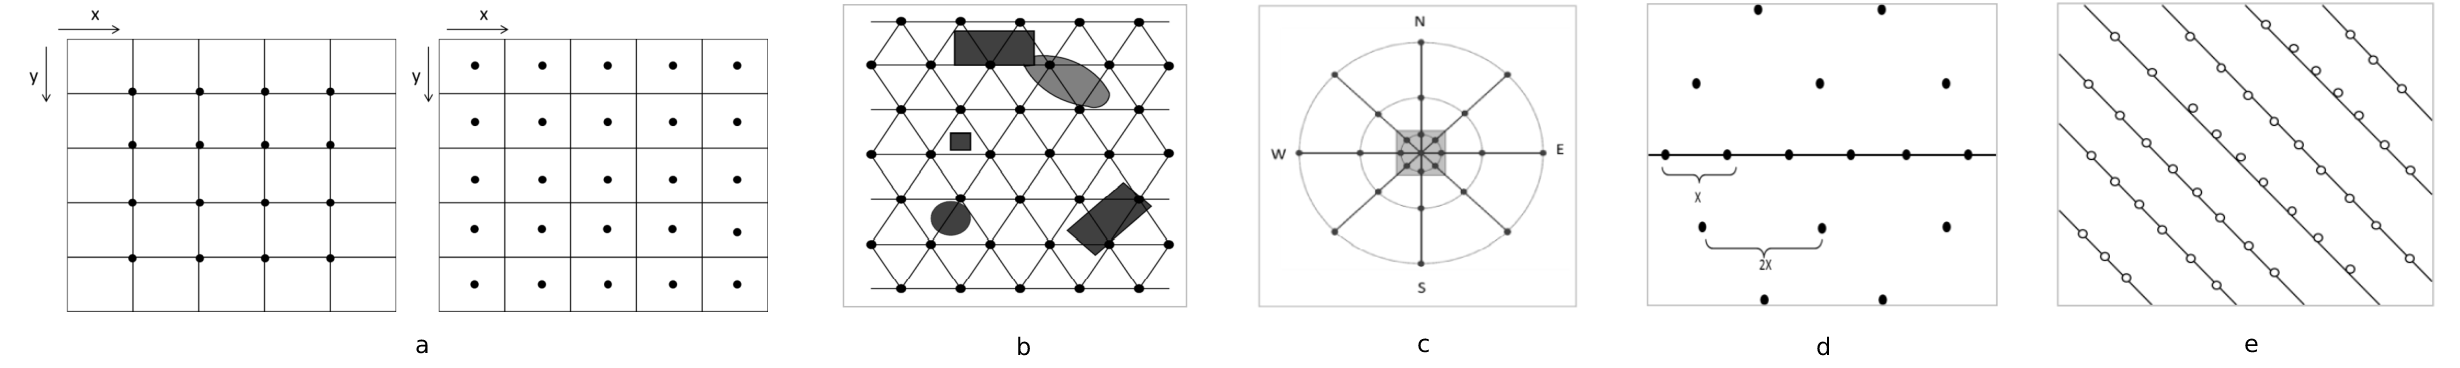
\includegraphics[width=0.3\paperwidth]{ref/uniform-sampling-patterns.png}
    \caption{Patrones de muestreo con distribución uniforme}
    a) Rejillas regulares, b) Rejillas triangulares, c) Rejilla circular, d) Sobre una línea, e) Diagonales múltiples \\
    Fuente: \textit{Guía de muestreo de suelo $\mid$ Gob.Pe} \cite{gobpe-ministerio-del-ambiente-2014}
\end{figure}


\subsubsection{Con Distribución Heterogénea}

Por último se enumeran este otro tipo de patrones que se pueden encontrar en un muestreo físico. Estos consisten en:

\begin{itemize}
    \item Diagonal simple
    \item Diagonales cruzadas rotantes
    \item Muestreo irregular en forma de N, S, X, o W
    \item Zig-zag
    \item Zig-zag transverso
\end{itemize}
